\documentclass[border=10pt]{standalone}
\usepackage[svgnames]{xcolor}
\usepackage{amsmath}
\usepackage{pgfplots}
\pgfplotsset{compat=newest}
\usepackage[sfdefault]{FiraSans}
\usepackage{FiraMono}
\renewcommand*\familydefault{\sfdefault}
\begin{document}
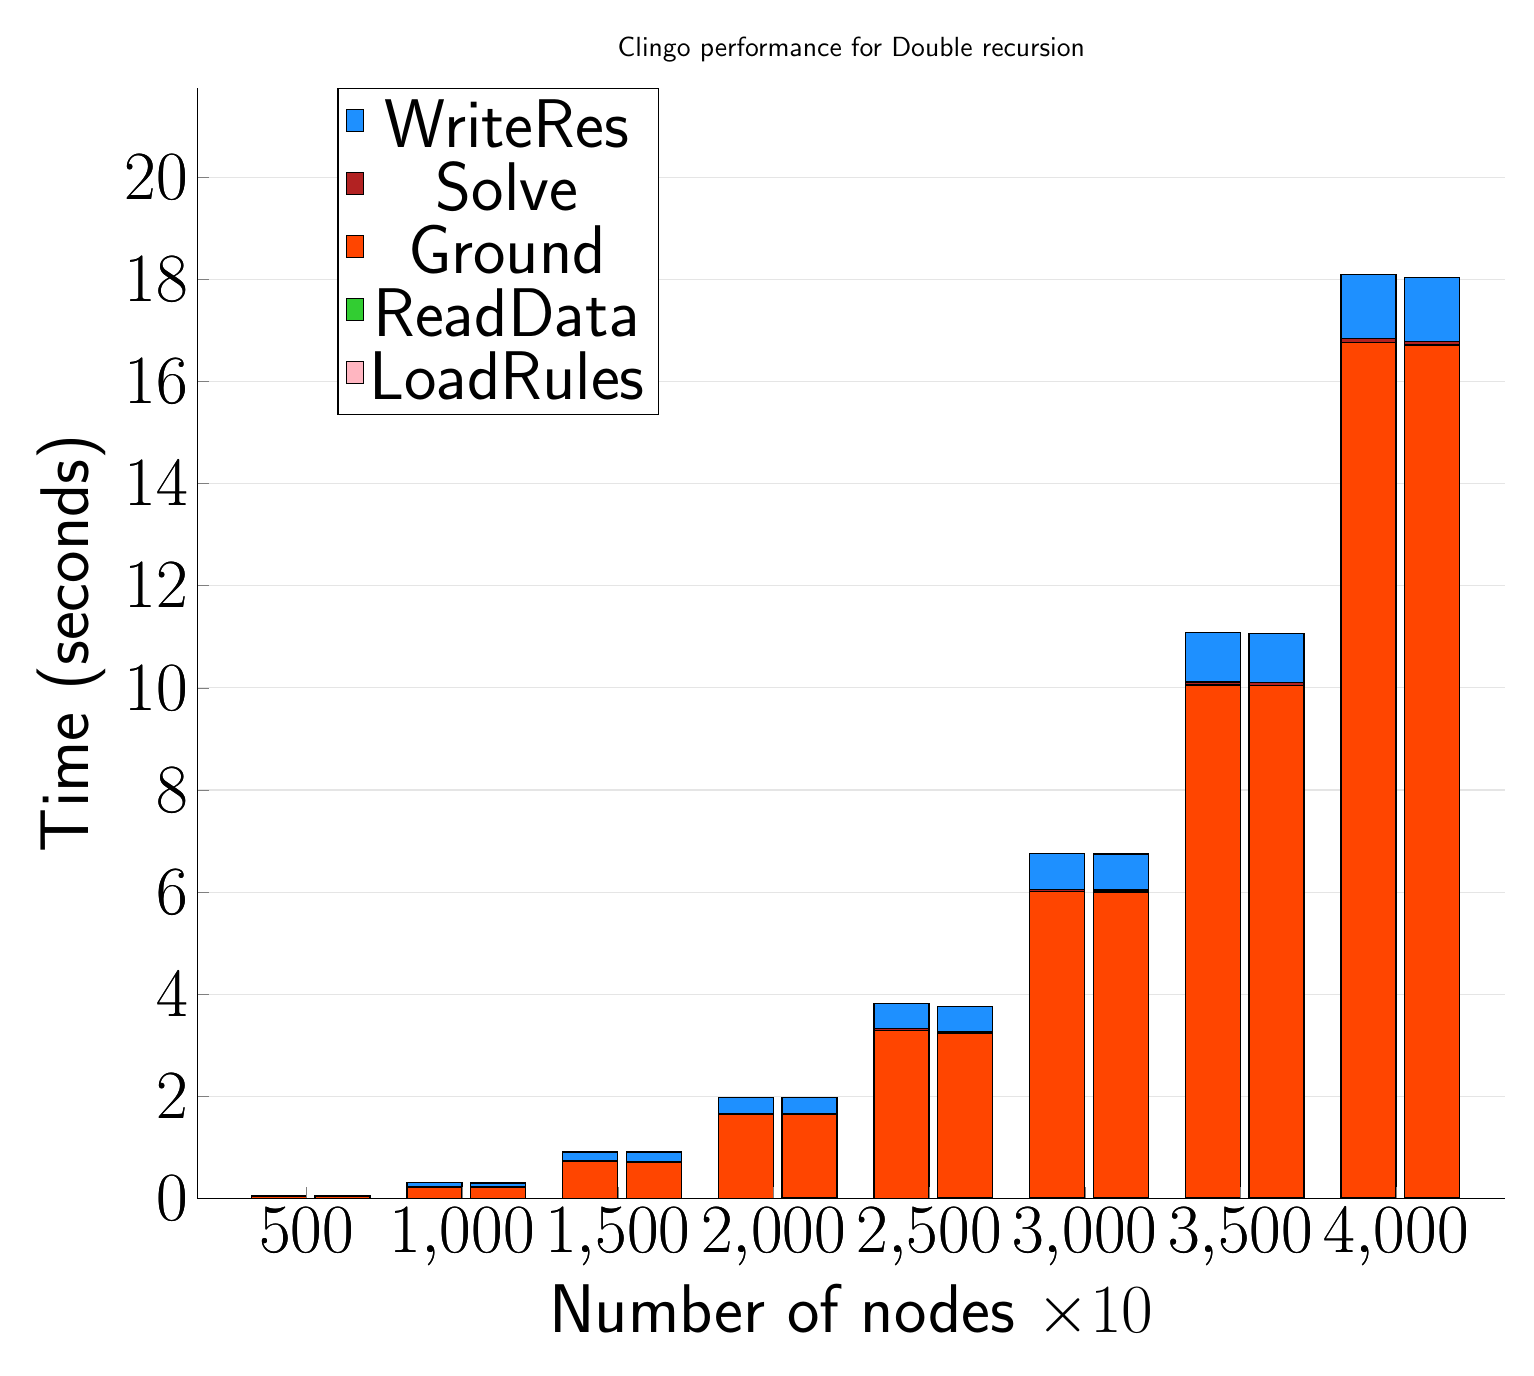
\begin{tikzpicture}
	\begin{axis}[
			ybar stacked,
			title={Clingo performance for Double recursion},
			bar shift=-10pt,
			width=1.5\textwidth,
			bar width=0.7cm,
			ymajorgrids, tick align=inside,
			major grid style={draw=gray!20},
			xtick=data,
			ymin=0, ymax=21.74900002479553,
			axis x line*=bottom,
			axis y line*=left,
			enlarge x limits=0.1,
			legend style={
					at={(0.23, 1)},
					anchor=north,
					legend columns=1,
					font=\Huge,
				},
			ylabel={Time (seconds)},
			xlabel={Number of nodes $\times 10$},
			label style={font=\Huge},
			tick label style={font=\Huge},
		]
		\addlegendimage{fill=DodgerBlue, draw=black, line width=0.2pt}
		\addlegendentry{WriteRes}
		\addlegendimage{fill=FireBrick, draw=black, line width=0.2pt}
		\addlegendentry{Solve}
		\addlegendimage{fill=OrangeRed, draw=black, line width=0.2pt}
		\addlegendentry{Ground}
		\addlegendimage{fill=LimeGreen, draw=black, line width=0.2pt}
		\addlegendentry{ReadData}
		\addlegendimage{fill=LightPink, draw=black, line width=0.2pt}
		\addlegendentry{LoadRules}
		\addplot +[fill=LightPink, draw=black, line width=0.5pt] coordinates {
				(500, 0.0)
				(1000, 0.0)
				(1500, 0.0)
				(2000, 0.0)
				(2500, 0.0)
				(3000, 0.0)
				(3500, 0.0)
				(4000, 0.0)
			};
		\addplot +[fill=LimeGreen, draw=black, line width=0.5pt] coordinates {
				(500, 0.0029999971389770507)
				(1000, 0.0029999971389770507)
				(1500, 0.003000020980834961)
				(2000, 0.004999995231628418)
				(2500, 0.0039999961853027345)
				(3000, 0.009999990463256836)
				(3500, 0.010000038146972656)
				(4000, 0.012000012397766113)
			};
		\addplot +[fill=OrangeRed, draw=black, line width=0.5pt] coordinates {
				(500, 0.03199999332427979)
				(1000, 0.22200000286102295)
				(1500, 0.7209999799728394)
				(2000, 1.644000029563904)
				(2500, 3.2929999351501467)
				(3000, 6.002999997138977)
				(3500, 10.044000029563904)
				(4000, 16.74900002479553)
			};
		\addplot +[fill=FireBrick, draw=black, line width=0.5pt] coordinates {
				(500, 0.0)
				(1000, 0.0029999971389770507)
				(1500, 0.01100001335144043)
				(2000, 0.018000006675720215)
				(2500, 0.031000041961669923)
				(3000, 0.043999981880187986)
				(3500, 0.061999964714050296)
				(4000, 0.08199996948242187)
			};
		\addplot +[fill=DodgerBlue, draw=black, line width=0.5pt] coordinates {
				(500, 0.023000001907348633)
				(1000, 0.08300001621246338)
				(1500, 0.17799999713897705)
				(2000, 0.31399996280670167)
				(2500, 0.48999996185302735)
				(3000, 0.7050000190734863)
				(3500, 0.9710000038146973)
				(4000, 1.247000026702881)
			};
	\end{axis}
	\begin{axis}[
			ybar stacked,
			bar shift=13pt,
			width=1.5\textwidth,
			bar width=0.7cm,
			ymajorgrids, tick align=inside,
			major grid style={draw=none},
			xtick=data,
			ymin=0, ymax=21.74900002479553,
			axis x line*=none,
			axis y line*=none,
			enlarge x limits=0.1,
			label style={font=\Huge},
			tick label style={font=\Huge},
		]
		\addplot +[fill=LightPink, draw=black, line width=0.5pt] coordinates {
				(500, 0.0)
				(1000, 0.0)
				(1500, 0.0)
				(2000, 0.0)
				(2500, 0.0)
				(3000, 0.0)
				(3500, 0.0)
				(4000, 0.0)
			};
		\addplot +[fill=LimeGreen, draw=black, line width=0.5pt] coordinates {
				(500, 0.0)
				(1000, 0.0)
				(1500, 0.003999999999999999)
				(2000, 0.009999999999999997)
				(2500, 0.009999999999999997)
				(3000, 0.008999999999999998)
				(3500, 0.009999999999999997)
				(4000, 0.009999999999999997)
			};
		\addplot +[fill=OrangeRed, draw=black, line width=0.5pt] coordinates {
				(500, 0.03799999999999999)
				(1000, 0.22400000000000003)
				(1500, 0.715)
				(2000, 1.6420000000000001)
				(2500, 3.2239999999999993)
				(3000, 5.990999999999999)
				(3500, 10.032)
				(4000, 16.701)
			};
		\addplot +[fill=FireBrick, draw=black, line width=0.5pt] coordinates {
				(500, 0.001999999999999999)
				(1000, 0.0050000000000000044)
				(1500, 0.01200000000000001)
				(2000, 0.017999999999999995)
				(2500, 0.031000000000000007)
				(3000, 0.04400000000000008)
				(3500, 0.062000000000000145)
				(4000, 0.07699999999999949)
			};
		\addplot +[fill=DodgerBlue, draw=black, line width=0.5pt] coordinates {
				(500, 0.018000000000000006)
				(1000, 0.07400000000000002)
				(1500, 0.181)
				(2000, 0.31100000000000005)
				(2500, 0.48999999999999994)
				(3000, 0.7009999999999998)
				(3500, 0.9649999999999996)
				(4000, 1.2430000000000003)
			};
	\end{axis}
\end{tikzpicture}

\end{document}
